\documentclass[aspectratio=169]{beamer}

% --- THEME AND STYLING ---
\usetheme{Madrid}
\useoutertheme{default}
\useinnertheme{rectangles}
\setbeamertemplate{navigation symbols}{}

% --- CUSTOM COLOR PALETTE ---
\definecolor{SkyBlue}{RGB}{135, 206, 235}
\definecolor{DarkNavy}{RGB}{0, 0, 139}
\definecolor{LightBlueBg}{RGB}{240, 248, 255}
\definecolor{AccentBlue}{RGB}{70, 130, 180}
\definecolor{DarkGreyText}{RGB}{50, 50, 50}
\definecolor{HighlightGreen}{RGB}{34, 139, 34}
\definecolor{AlertRed}{RGB}{220, 20, 60}

\setbeamercolor{palette primary}{bg=SkyBlue,fg=DarkNavy}
\setbeamercolor{palette secondary}{bg=DarkNavy,fg=white}
\setbeamercolor{palette tertiary}{bg=AccentBlue,fg=white}
\setbeamercolor{palette quaternary}{bg=SkyBlue,fg=DarkNavy}
\setbeamercolor{structure}{fg=DarkNavy}
\setbeamercolor{section in toc}{fg=DarkNavy}
\setbeamercolor{frametitle}{bg=SkyBlue,fg=DarkNavy}
\setbeamercolor{block title}{bg=DarkNavy,fg=white}
\setbeamercolor{block body}{bg=LightBlueBg,fg=DarkGreyText}
\setbeamercolor{block title alerted}{bg=AlertRed,fg=white}
\setbeamercolor{block body alerted}{bg=LightBlueBg,fg=DarkGreyText}
\setbeamercolor{block title example}{bg=HighlightGreen,fg=white}
\setbeamercolor{block body example}{bg=LightBlueBg,fg=DarkGreyText}
\setbeamertemplate{footline}[frame number]
\setbeamercolor{footline}{fg=DarkNavy}
\setbeamertemplate{blocks}[rounded][shadow=false]

% --- PACKAGES ---
\usepackage[utf8]{inputenc}
\usepackage{amsmath,amssymb}
\usepackage{booktabs}
\usepackage{graphicx}
\usepackage{array}
\usepackage{multirow}
\usepackage{tikz}
\usepackage{siunitx}

% --- TITLE PAGE ---
\title[Sustainable Rendezvous]{Sustainable "Rendezvous": A Festival Systems Challenge}
\subtitle{Comprehensive Process Optimization (Modules 3.1 - 3.4)}
\author[Team Sustainability]{Sustainability Task Force}
\institute{Department of Chemical Engineering\\
\vspace{0.2cm}
\small Course: CLL782 - Process Optimization\\
\small Instructor: Prof. Om Prakash}
\date{\today}

\begin{document}

% --- TITLE SLIDE ---
\begin{frame}[plain]
    \titlepage
    \vspace{-0.5cm}
    \begin{center}
        \small Presented by: Yash
    \end{center}
\end{frame}

% --- OUTLINE ---
\begin{frame}{Outline}
    \tableofcontents[hideallsubsections]
\end{frame}

%%%%%%%%%%%%%%%%%%%%%%%%%%%%%%%%%%%%%%%%%%%%%%%%%%%%%%%%%%%%%%%%%
\section{1. Introduction \& Scope}
%%%%%%%%%%%%%%%%%%%%%%%%%%%%%%%%%%%%%%%%%%%%%%%%%%%%%%%%%%%%%%%%%

\begin{frame}{The Challenge: Greening Asia's Largest Fest}
    \begin{columns}[T]
        \begin{column}{0.55\textwidth}
            \begin{block}{Context}
                \begin{itemize}
                    \item \textbf{Rendezvous (IIT Delhi)}: $\sim$160,000 attendees over 4 days.
                    \item \textbf{Problem}: Massive environmental footprint (Waste, Energy, Carbon).
                    \item \textbf{Goal}: Use Process Optimization to model and minimize this Environmental Load ($E$).
                \end{itemize}
            \end{block}

            \begin{alertblock}{Scope: High-Intensity Zone}
                \begin{itemize}
                    \item \textbf{Area}: $\sim$82-90 Acres (26\% of Campus).
                    \item \textbf{Locations}: OAT, Nalanda, SAC, LHC, Red Square.
                    \item \textbf{Footfall}: Captures 90\% of event intensity.
                \end{itemize}
            \end{alertblock}
        \end{column}

        \begin{column}{0.40\textwidth}
            \centering
            % Placeholder for map if available, or text
            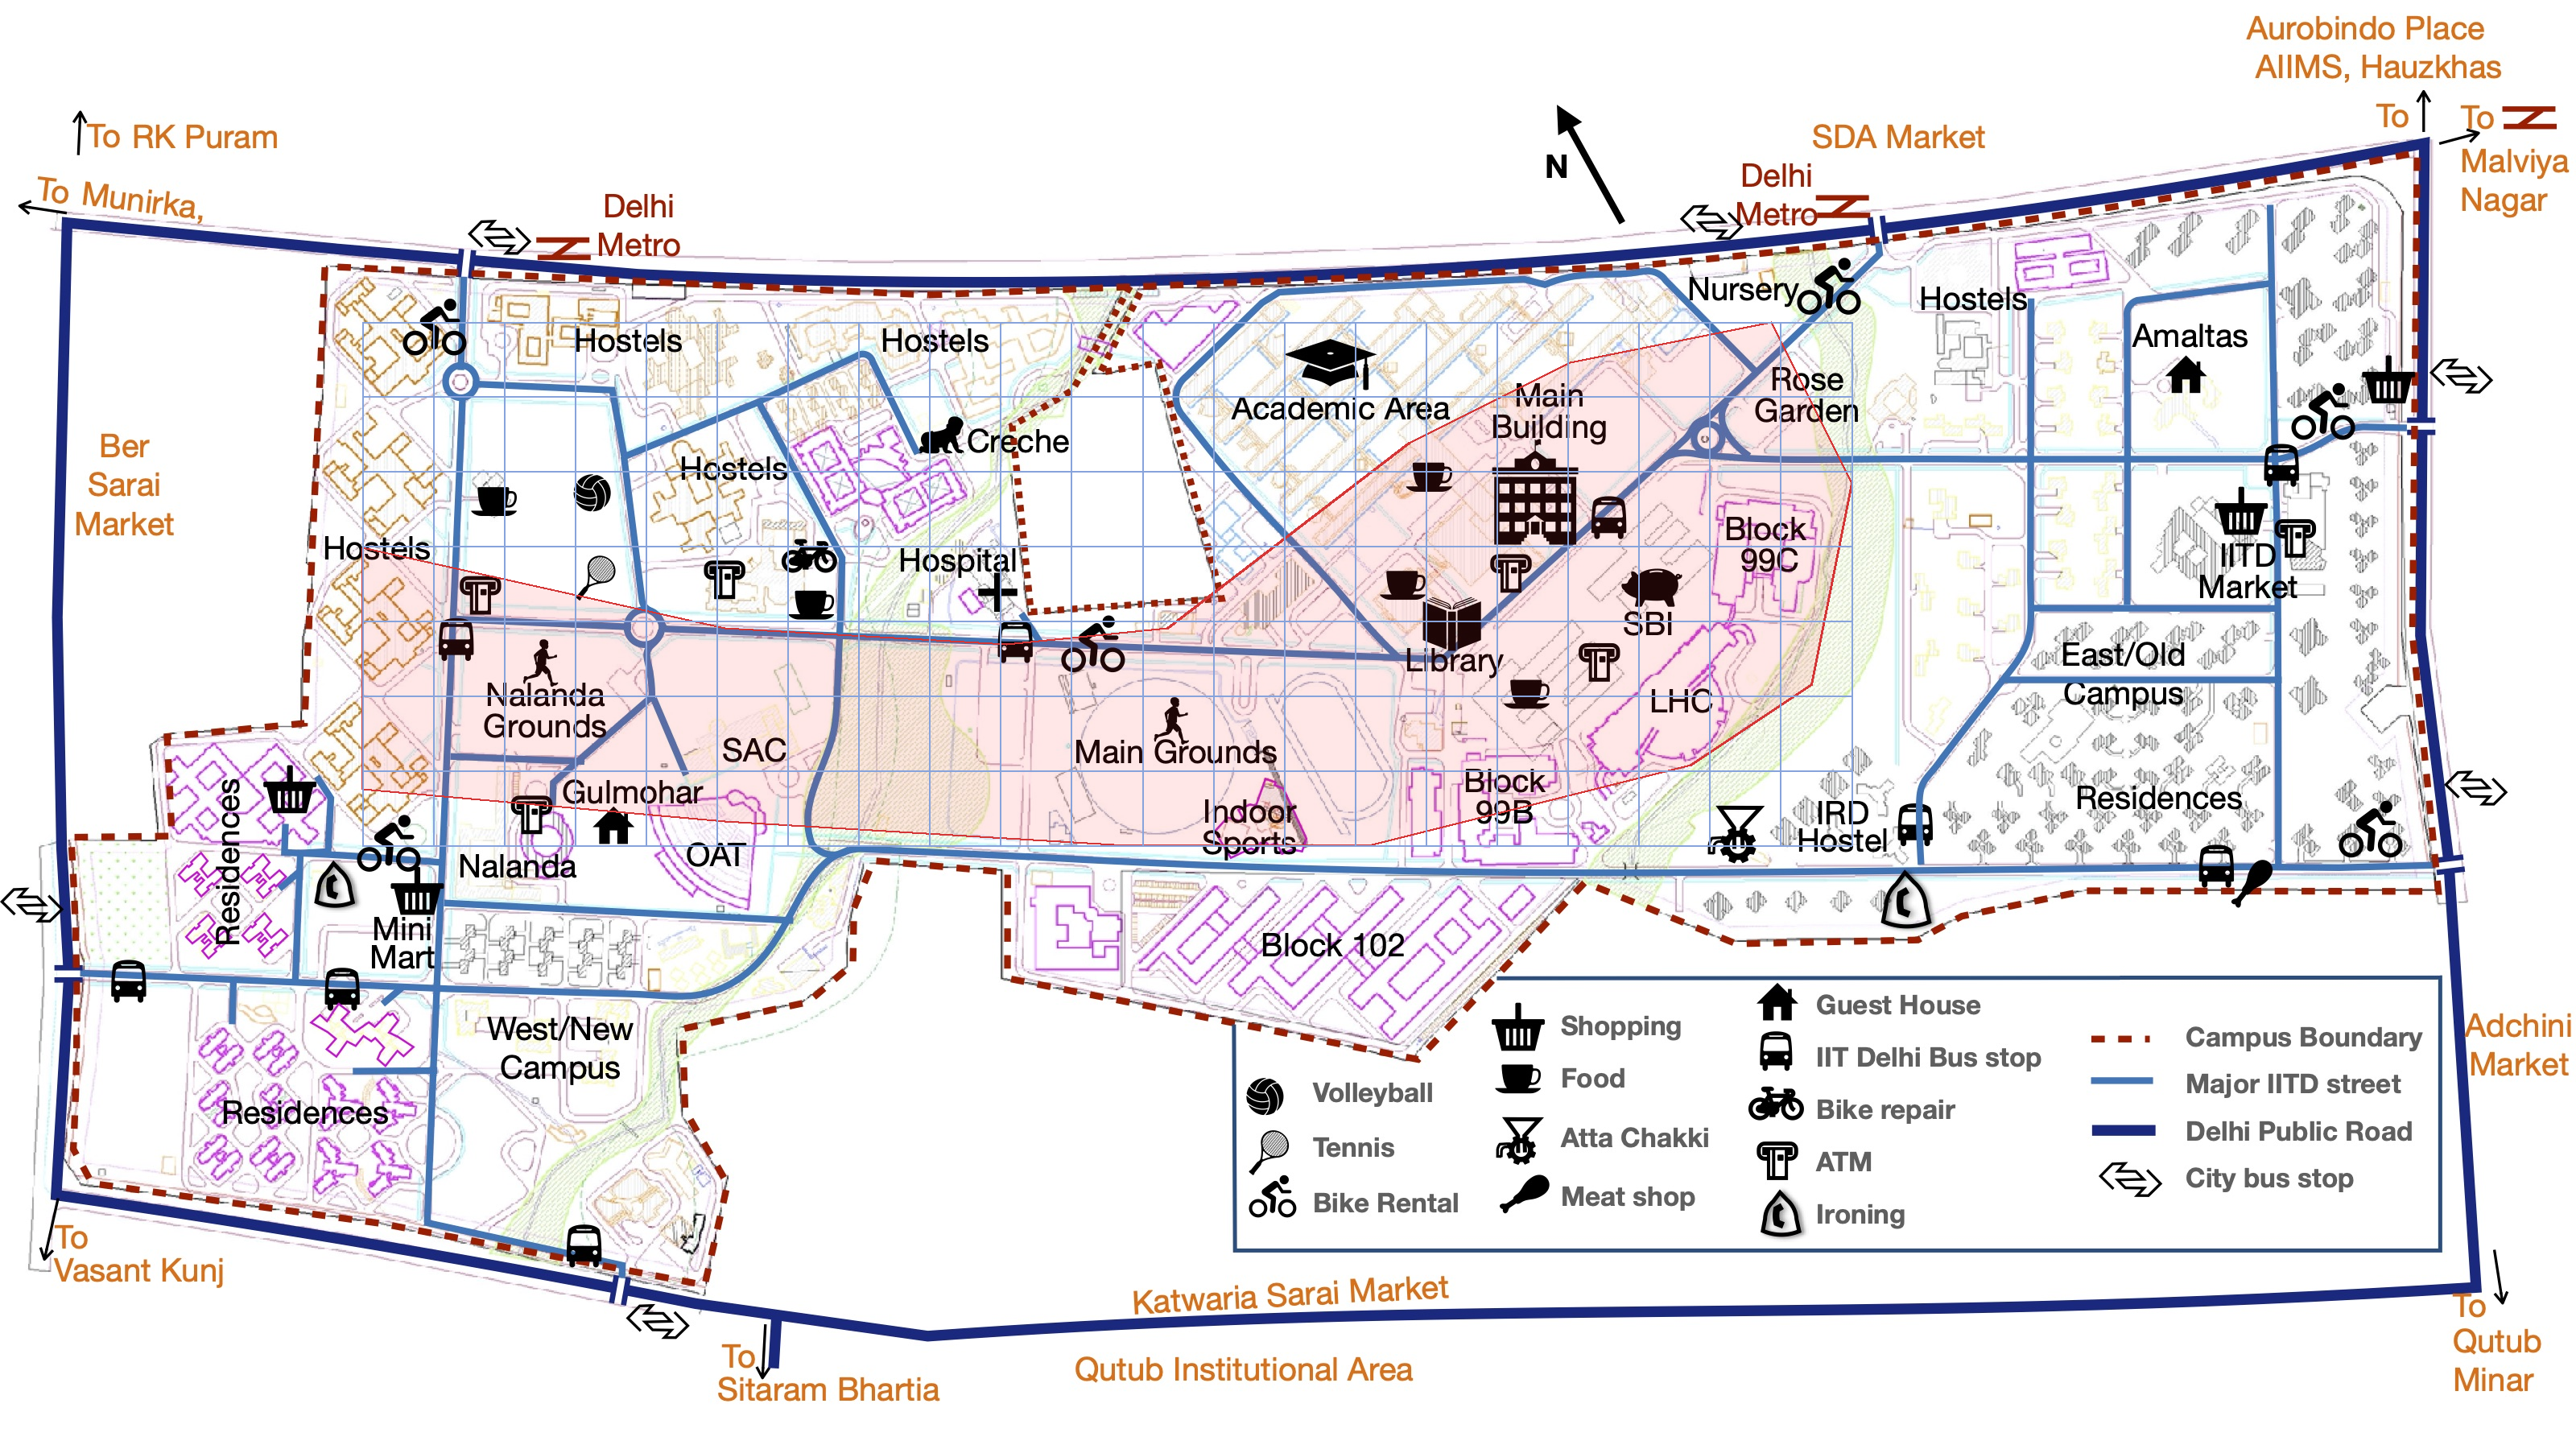
\includegraphics[width=0.95\textwidth]{../Module_3_1/iitd_roi_grid_map.jpg} \\
            \scriptsize{Target ROI: 82 Acres, 137 Grid Cells}
        \end{column}
    \end{columns}
\end{frame}

%%%%%%%%%%%%%%%%%%%%%%%%%%%%%%%%%%%%%%%%%%%%%%%%%%%%%%%%%%%%%%%%%
\section{2. Module 3.1: Environmental Load Modeling}
%%%%%%%%%%%%%%%%%%%%%%%%%%%%%%%%%%%%%%%%%%%%%%%%%%%%%%%%%%%%%%%%%

\begin{frame}{3.1 Problem Statement \& Methodology}
    \textbf{Problem:} Develop a mathematical function to Quantify Total Environmental Load ($E$).

    \vspace{0.3cm}
    \begin{block}{Key Variables}
        \begin{tabular}{l l l l}
            \textbf{Sym} & \textbf{Description} & \textbf{Type} & \textbf{Value/Range} \\
            \midrule
            $N$ & Number of Attendees & Demand & 160,000 (Total) \\
            $S$ & Number of Stalls & Decision & $100 - 300$ \\
            $A$ & Activity Hours & Decision & 4 Days $\times$ 12 hrs \\
        \end{tabular}
    \end{block}

    \vspace{0.2cm}
    \textbf{Assumed Constants (Ref: Literature/IITD Data):}
    \begin{itemize}
        \item Base Impact $\alpha_1$: 2.5 kg CO$_2$/person.
        \item Stall Impact $\alpha_2$: 18 kg CO$_2$/stall (Embodied).
        \item Congestion Penalty $\gamma_{NS}$: 0.0005 (Waste leakage factor).
    \end{itemize}
\end{frame}

\begin{frame}{3.1 Formulation \& Results}
    \begin{alertblock}{Objective Function: Minimize Load $E$}
        $$ E = \underbrace{(\alpha_1 N + \alpha_2 S)}_{\text{Base}} + \underbrace{(\beta_N N^{1.3})}_{\text{Non-linear Scale}} + \underbrace{\left( \gamma_{NS} \frac{N^2}{S} \right)}_{\text{Congestion Penalty}} $$
    \end{alertblock}
    
    \vspace{0.3cm}
    \textbf{Preliminary Insight:}
    \begin{itemize}
        \item The term $N^2/S$ represents littering caused by overcrowding/queues.
        \item \textbf{Optimization}: $\frac{dE}{dS} = 0 \implies S^* = N \sqrt{\frac{\gamma_{NS}}{\alpha_2}}$
        \item For $N=40,000$/day, $\alpha_2=18$, $\gamma_{NS}=0.0005$ $\rightarrow$ \textbf{$S^* \approx 210$ Stalls}.
        \item \textit{Current scenario ($\sim$100 stalls) is suboptimal due to high congestion penalty.}
    \end{itemize}
\end{frame}

%%%%%%%%%%%%%%%%%%%%%%%%%%%%%%%%%%%%%%%%%%%%%%%%%%%%%%%%%%%%%%%%%
\section{3. Module 3.2: Dustbin Placement (FLP)}
%%%%%%%%%%%%%%%%%%%%%%%%%%%%%%%%%%%%%%%%%%%%%%%%%%%%%%%%%%%%%%%%%

\begin{frame}{3.2 Problem Statement \& Variables}
    \textbf{Problem:} Optimal placement of dustbins to minimize user inconvenience (walking distance) and littering.
    
    \begin{block}{Variable Description}
        \begin{itemize}
            \item $i$: Demand Zones (Grid Cells).
            \item $j$: Candidate Bin Locations.
            \item $y_{j,t} \in \{0,1\}$: Binary decision to install bin type $t$ at loc $j$.
            \item $a_{i,j,t} \in [0,1]$: Fraction of demand from $i$ assigned to $j$.
        \end{itemize}
    \end{block}

    \textbf{Constants:}
    \begin{itemize}
        \item \textbf{Waste Rate ($w$)}: 0.15 kg/person/visit (Food fest norm).
        \item \textbf{Service Radius ($R_t$)}: 30m (High Intensity) to 50m (Pathways).
        \item \textbf{Bin Capacity ($K_t$)}: 20-30 kg (Dual FRP Bins).
    \end{itemize}
\end{frame}

\begin{frame}{3.2 Mathematical Formulation}
    \begin{exampleblock}{Objective: Minimize Total Inconvenience $Z$}
        $$ \text{Min } Z = \sum_{i} \sum_{j} \sum_{t} \left( F_i \cdot a_{i,j,t} \cdot D_{ij} \right) $$
    \end{exampleblock}

    \textbf{Subject to Constraints:}
    \begin{enumerate}
        \item \textbf{Coverage}: $\sum_{j,t} a_{i,j,t} = 1$ (All waste must be collected).
        \item \textbf{Capacity}: $\sum_{i} (F_i \cdot w \cdot a_{i,j,t}) \le K_t \cdot y_{j,t}$ (Bins can't overflow).
        \item \textbf{Radius (Accessibility)}: $a_{i,j,t} = 0$ if $D_{ij} > R_t$.
        \item \textbf{Budget}: $\sum_{j,t} C_t \cdot y_{j,t} \le B$.
    \end{enumerate}
\end{frame}

%%%%%%%%%%%%%%%%%%%%%%%%%%%%%%%%%%%%%%%%%%%%%%%%%%%%%%%%%%%%%%%%%
\section{4. Module 3.3: Waste Logistics (Network Flow)}
%%%%%%%%%%%%%%%%%%%%%%%%%%%%%%%%%%%%%%%%%%%%%%%%%%%%%%%%%%%%%%%%%

\begin{frame}{3.3 Problem Statement \& Hierarchy}
    \textbf{Problem:} Design a logicstics network to transport 6,000 kg/day of waste from zones to processing units.
    
    \vspace{0.2cm}
    \textbf{System Components:}
    \begin{itemize}
        \item \textbf{Sources ($i$)}: 90-acre ROI zones.
        \item \textbf{Sinks ($j$)}: Biogas (On-campus), Okhla Landfill, Recyclers.
        \item \textbf{Vehicles ($k$)}: Small Tippers (Tata Ace EV).
    \end{itemize}

    \begin{block}{Parameters \& Constants}
        \begin{itemize}
            \item \textbf{Vehicle Capacity ($V_{cap}$)}: 750 kg.
            \item \textbf{Fixed Cost ($C_{fixed}$)}: Rs.800/vehicle/day.
            \item \textbf{Variable Cost}: Rs.20/km.
        \end{itemize}
    \end{block}
\end{frame}

\begin{frame}{3.3 Formulation (Min Cost Flow)}
    \begin{alertblock}{Objective: Minimize Total Logistics Cost}
        $$ \text{Min } Z = \underbrace{\sum_{i,j} x_{i,j} (C_{dist} D_{ij} + C_{proc,j})}_{\text{Variable Cost}} + \underbrace{C_{fixed} \cdot \left\lceil \frac{\sum x_{i,j}}{V_{cap}} \right\rceil}_{\text{Fixed Fleet Cost}} $$
    \end{alertblock}

    \textbf{Constraints:}
    \begin{enumerate}
        \item \textbf{Supply}: $\sum_j x_{i,j} = \text{Waste Generated}_i$.
        \item \textbf{Throughput}: $\sum_i x_{i,j} \le \text{Capacity}_j$ (e.g., Biogas limit).
        \item \textbf{Fleet}: Total volume $\le$ Number of vehicles $\times V_{cap}$.
    \end{enumerate}
\end{frame}

%%%%%%%%%%%%%%%%%%%%%%%%%%%%%%%%%%%%%%%%%%%%%%%%%%%%%%%%%%%%%%%%%
\section{5. Module 3.4: Water Refill Stations}
%%%%%%%%%%%%%%%%%%%%%%%%%%%%%%%%%%%%%%%%%%%%%%%%%%%%%%%%%%%%%%%%%

\begin{frame}{3.4 Problem Statement \& Setup}
    \textbf{Problem:} Plan water refill stations to support reusable bottle policy (Zero Plastic).
    
    \begin{block}{Variables}
        \begin{itemize}
            \item $y_j \in \{0, 1\}$: Install Station at location $j$?
            \item $x_{i,j} \in [0, 1]$: Fraction of demand satisfied by $j$.
        \end{itemize}
    \end{block}

    \textbf{Assumptions \& Constants:}
    \begin{itemize}
        \item \textbf{Demand ($d_i$)}: 0.25 L/hr/person $\rightarrow$ 10,000 LPH Peak.
        \item \textbf{Station Capacity}: 250 LPH (Cooling rate bottleneck).
        \item \textbf{Cost of Walking ($C_{walk}$)}: Rs.0.02 per meter (Time value).
        \item \textbf{Install Cost ($f_j$)}: Rs.1,00,000 (RO + Cooling).
    \end{itemize}
\end{frame}

\begin{frame}{3.4 Formulation (Capacitated P-Median)}
    \begin{exampleblock}{Objective: Min Generalized Cost}
        $$ \text{Min } Z = \underbrace{\sum_{j} f_j y_j}_{\text{Installation Cost}} + \underbrace{\sum_{i,j} (d_i x_{i,j}) D_{ij} C_{walk}}_{\text{User Inconvenience Cost}} $$
    \end{exampleblock}

    \textbf{Key Constraints:}
    \begin{enumerate}
        \item \textbf{Demand Met}: $\sum_j x_{i,j} = 1$.
        \item \textbf{Capacity}: $\sum_i d_i x_{i,j} \le \text{Cap}_j \cdot y_j$.
        \item \textbf{Logical}: User can only go to $j$ if $y_j=1$.
    \end{enumerate}
    
    \vspace{0.2cm}
    \textit{Trade-off: More stations = Higher Install Cost vs. Less User Walking.}
\end{frame}

%%%%%%%%%%%%%%%%%%%%%%%%%%%%%%%%%%%%%%%%%%%%%%%%%%%%%%%%%%%%%%%%%
\section{Conclusion}
%%%%%%%%%%%%%%%%%%%%%%%%%%%%%%%%%%%%%%%%%%%%%%%%%%%%%%%%%%%%%%%%%

\begin{frame}{Conclusion}
    \begin{block}{Integrated Sustainability Strategy}
        \begin{enumerate}
            \item \textbf{Mod 3.1}: Optimize Scale ($S^* \approx 210$) to reduce congestion-led waste.
            \item \textbf{Mod 3.2}: Place Bins within 30m radius to capture waste at source.
            \item \textbf{Mod 3.3}: Efficient Logistics routing to minimize transport carbon.
            \item \textbf{Mod 3.4}: Strategic Water Stations to eliminate plastic bottles.
        \end{enumerate}
    \end{block}
    
    \centering
    \vspace{0.5cm}
    \LARGE \textbf{Technological Optimism + Process Optimization \\ = Greener Rendezvous}
\end{frame}

\begin{frame}[plain]
    \vfill
    \begin{center}
        {\Huge \textcolor{DarkNavy}{Thank You}} \\
        \vspace{1cm}
        \small Open Loop: Optimizing "Rendezvous" \\
        \small Dept of Chemical Engineering, IIT Delhi
    \end{center}
    \vfill
\end{frame}

\end{document}
